\documentclass{standalone}

\usepackage{tikz}
\usetikzlibrary{arrows,backgrounds,er,shapes,chains}

\begin{document}
  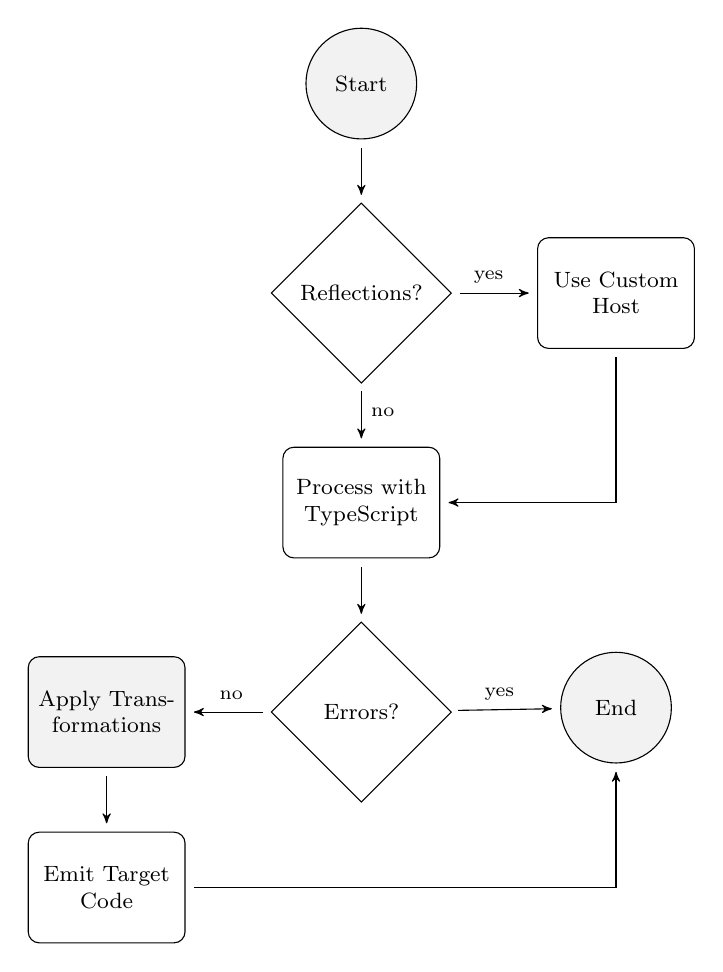
\begin{tikzpicture}[
    ->,
    >=stealth',
    shorten >= 1pt,
    auto,
    node distance=2.3em and 3.5em,
    font=\footnotesize,
    text centered,
    every entity/.style={
      minimum width=7.2em,
  	   minimum height=4.3em,
      outer sep=0,
      inner sep=.1em
    }
  ]
    
  \tikzstyle{decision} = [diamond, draw, text width=4.5em, minimum height=6.5em, minimum width=6.5em, node distance=2.3em and 2.3em, text badly centered, inner sep=.1em, outer sep=0]
  \tikzstyle{block} = [rectangle, draw, text width=5em, text centered, rounded corners, minimum height=4em]
  \tikzstyle{std} = [rectangle, draw, text width=5em, text centered, minimum height=4em]
  \tikzstyle{line} = [draw, -latex']
  \tikzstyle{cloud} = [draw, ellipse, minimum height=2em]
  \tikzstyle{round} = [draw, circle, inner sep=0.5em, minimum size=4em]
    

  \node [round, fill=gray!10] (start) {Start};
  \node [decision, below=of start] (reflections) {Reflections?};

  \path[shorten >=0.3em, shorten <=0.3em,->] (start) edge node {} (reflections);

  \node [block, right=of reflections, xshift=-0.4em] (host) {Use Custom Host};
  \node [block, draw=none, below=of host, yshift=-1.2em] (spacer) {};
  \node [block, below=of reflections] (program) {Process with TypeScript};

  \path[shorten >=0.3em, shorten <=0.3em,->] (reflections) edge node[xshift=-0.2em] {\scriptsize{yes}} (host);
  \path[shorten >=0.3em, shorten <=0.3em,->] (reflections) edge node[yshift=0.1em] {\scriptsize{no}} (program);
  \draw[shorten >=0.3em,shorten <=0.3em,->] (host.south) -- ++(0,-2.0em) |-  (program.east);

  \node [decision, below=of program] (errors) {Errors?};
  \node [block, left=of errors, xshift=0.4em, fill=gray!10] (transform) {Apply Transformations};
  \node [round, below=of spacer, yshift=-1.1em, fill=gray!10] (end) {End};

  \path[shorten >=0.3em, shorten <=0.3em,->] (program) edge node {} (errors);
  \path[shorten >=0.3em, shorten <=0.3em,->] (errors) edge node[xshift=-0.2em] {\scriptsize{yes}} (end);
  \path[shorten >=0.3em, shorten <=0.3em,->] (errors) edge node[yshift=1.1 em, xshift=0.1em] {\scriptsize{no}} (transform);

  \node [block, below=of transform] (emit) {Emit Target Code};

  \path[shorten >=0.3em, shorten <=0.3em,->] (transform) edge node {} (emit);
  \draw[shorten >=0.3em,shorten <=0.3em,->] (emit.east) -- ++(0.3em, 0) -|  (end.south);
    
  \end{tikzpicture}
\end{document}
